% ========================================================
%  Flow-Guided Priority Shielding for Continuous-Space MAPF
%  ICRA submission --- IEEEtran two-column format
%
%  Compile from the paper/ directory:
%    cd paper
%    pdflatex main && bibtex main && pdflatex main && pdflatex main
%
%  Adapting to CoRL / NeurIPS / ICLR:
%    Swap \documentclass + author block for the venue template.
%    All \input{sections/...} files are venue-agnostic.
% ========================================================
\documentclass[conference]{IEEEtran}

% ---- Packages ------------------------------------------
\usepackage[utf8]{inputenc}
\usepackage[T1]{fontenc}
\usepackage{amsmath,amssymb,amsfonts}
\usepackage{graphicx}
\usepackage{booktabs}
\usepackage{cite}
\usepackage{url}
\usepackage[hidelinks]{hyperref}
\usepackage{xcolor}
\usepackage{microtype}
\usepackage{algorithm2e}
\usepackage{bm}
\usepackage{multirow}
\usepackage{array}

% ---- algorithm2e style ---------------------------------
\SetAlFnt{\small}
\SetAlCapFnt{\small}
\SetAlCapNameFnt{\small}
\RestyleAlgo{ruled}

% ---- Suppress extra space after periods ----------------
\frenchspacing

% ========================================================
\begin{document}

\title{Flow-Guided Priority Shielding for\\Continuous-Space Multi-Agent Path Finding}

\author{%
  \IEEEauthorblockN{Author Names}
  \IEEEauthorblockA{Institution Name\\
    City, Country\\
    email@institution.edu}
}

\maketitle

% --------------------------------------------------------
\begin{abstract}
Continuous-space Multi-Agent Path Finding (MAPF) requires agents to navigate to individual goals in shared physical space while avoiding collisions. Classical velocity-obstacle methods such as ORCA suffer from symmetric deadlocks under high agent density. We introduce \textbf{EPIBTShield}, a continuous-space generalization of the discrete Priority Inheritance with Backtracking (PIBT) algorithm, which resolves velocity conflicts via dynamic priority ordering, a scored set of 19 candidate velocities per agent, and recursive backtracking up to depth~3. We pair EPIBTShield with a rectified-flow Graph Neural Network (GNN) that predicts spatially-informed preferred velocities from egocentric local observations and a dynamic neighbor communication graph, trained on EECBS expert demonstrations. On dense random maps with 100 agents over 512 steps, the combined system achieves $0.874$ fraction of agents at goal --- a 70.6 percentage-point improvement over ORCA --- with substantially fewer collisions. We characterize OOD failure on warehouse environments, isolating the learned flow component as the generalization bottleneck, and confirm low training variance across five random seeds.
\end{abstract}

% --------------------------------------------------------
% Introduction
\section{Introduction}
\label{sec:intro}

Multi-Agent Path Finding (MAPF) asks for a set of collision-free paths for a group of agents navigating from their respective start configurations to goal configurations~\cite{stern2019mapfsurvey}. Classical MAPF operates on graphs, where agents occupy discrete nodes and move along edges in synchronized time steps. This abstraction enables powerful algorithmic solutions such as Conflict-Based Search (CBS)~\cite{sharon2015cbs} and Priority Inheritance with Backtracking (PIBT)~\cite{okumura2022pibt}, but it imposes a fundamental mismatch with physical deployments: real robots move through continuous space with bounded velocities, non-trivial body radii, and smooth kinematic constraints that discrete graph abstractions cannot faithfully represent.

Continuous-space MAPF requires every agent to simultaneously (i) generate a kinematically feasible trajectory toward its goal and (ii) ensure that no two agents occupy overlapping regions at any point in time. Classical continuous approaches such as Optimal Reciprocal Collision Avoidance (ORCA)~\cite{vandenberg2011orca} and its predecessors~\cite{vandenberg2008rvo} handle the collision avoidance problem via local velocity-space constraints, but they optimize myopically, ignoring global path structure. Under high agent density, ORCA frequently deadlocks because no single agent can satisfy all its velocity constraints simultaneously. Learning-based methods that predict preferred velocities can improve global coordination~\cite{sartoretti2019primal,ma2021dhc,wang2023scrimp}, but without a hard safety layer, they accumulate collisions especially in dense or unseen environments.

This paper addresses the gap between expressive learned motion planning and rigorous conflict resolution in continuous space. We make two primary contributions. First, we introduce \textbf{EPIBTShield}, a continuous-space generalization of the discrete PIBT algorithm~\cite{okumura2022pibt}. EPIBTShield maintains a dynamic priority ordering over agents and resolves velocity conflicts by selecting from a scored discrete set of candidate velocities in strict priority order, with recursive backtracking to avoid global deadlock. Unlike ORCA, EPIBTShield does not require the velocity obstacle set to be non-empty; it always produces a valid (possibly zero) velocity for every agent while respecting hard geometric collision constraints. Second, we train a \textbf{rectified-flow GNN} that maps each agent's egocentric local observation to a preferred velocity. The network is conditioned on a graph of neighboring agents and is trained via flow matching~\cite{liu2023rectifiedflow,lipman2023flowmatching} to imitate expert trajectories generated by the EECBS planner~\cite{li2021eecbs}. These preferred velocities serve as inputs to EPIBTShield, providing goal-directed, spatially-aware guidance that substantially reduces the reliance on the shield's fallback candidates.


Our empirical evaluation spans four map types and two agent counts drawn from the MovingAI benchmark suite~\cite{sturtevant2012movingai}. On the primary in-distribution benchmark (random-32-32-10, $N=100$), the combined \mbox{Flow+EPIBTShield} system achieves an AtGoal fraction of $0.874$, compared to $0.168$ for ORCA and $0.486$ for a flow model shielded by ORCA — a gap of $70.6$ percentage points over the strongest pure-ORCA baseline. We also report honestly on the system's limitations: in warehouse-style out-of-distribution maps, the learned flow component underperforms a simple straight-line preferred velocity, suggesting that the generalization of the flow model is bounded by the distribution of its training demonstrations.

\subsection*{Summary of Contributions}

\begin{enumerate}
  \item \textbf{EPIBTShield}: a continuous-space velocity-conflict resolution algorithm that extends PIBT~\cite{okumura2022pibt} to continuous domains via dynamic priority ordering, a cosine-aligned candidate-velocity set with $19$ candidates per agent, and recursive backtracking up to depth~3.

  \item \textbf{Rectified-flow GNN}: a six-layer GraphSAGE~\cite{hamilton2017graphsage} network with egocentric CNN feature extraction, trained with rectified flow~\cite{liu2023rectifiedflow} on EECBS~\cite{li2021eecbs} expert demonstrations, that predicts spatially-informed preferred velocities for EPIBTShield.

  \item \textbf{Empirical evaluation} on MovingAI benchmarks~\cite{sturtevant2012movingai} demonstrating $70.6$\,pp improvement over ORCA in dense random maps, with systematic ablations and an honest analysis of OOD failure modes and multi-seed training variance.
\end{enumerate}

The paper is organized as follows. Section~\ref{sec:related} reviews related work. Section~\ref{sec:method} describes EPIBTShield and the flow GNN in detail. Section~\ref{sec:experiments} presents quantitative results and ablations. Section~\ref{sec:conclusion} concludes.

% Related Work
\section{Related Work}
\label{sec:related}

\subsection{Classical MAPF and Continuous Extensions}

The MAPF literature is extensive; we refer to Stern et al.~\cite{stern2019mapfsurvey} for a survey. CBS~\cite{sharon2015cbs} finds optimal solutions on graphs by splitting constraints upon conflict detection, and EECBS~\cite{li2021eecbs} extends this to bounded-suboptimal planning with inadmissible heuristics. PIBT~\cite{okumura2022pibt} is an incomplete but highly scalable priority-based method for iterative MAPF that resolves conflicts by recursively reassigning priorities; LaCAM~\cite{okumura2023lacam} further augments this with learning-based guidance. MAPF-LNS2~\cite{li2022mapflns2} achieves scalability through large-neighborhood search repair. These methods operate on discrete graphs and do not directly transfer to continuous kinematics.

Continuous-space MAPF has received comparatively less attention from the algorithmic community. Andreychuk and Yakovlev~\cite{andreychuk2019ccbs} extend CBS to continuous time, allowing agents to move at arbitrary speeds along grid edges, reducing artificial conflicts caused by time-step synchronization. However, this still assumes discrete spatial graphs. Our work operates in fully continuous 2D space with finite agent radii.

\subsection{Velocity Obstacle Methods}

Reciprocal Velocity Obstacles (RVO)~\cite{vandenberg2008rvo} introduced the idea of constraining each agent's velocity choice to lie outside the reciprocal velocity obstacle of each neighbor. ORCA~\cite{vandenberg2011orca} linearizes these constraints and uses a linear program to find the minimum-deviation feasible velocity, distributing collision-avoidance responsibility equally between agent pairs. The social force model~\cite{helbing1995socialforce} instead applies attractive and repulsive forces and has been influential in pedestrian simulation. Both approaches are purely reactive and local: they have no notion of global path coordination and are prone to symmetric deadlocks under high agent density, where agents block each other in a cycle. EPIBTShield addresses this via strict priority ordering, breaking symmetry by design.

\subsection{Learning-Based MAPF}

PRIMAL~\cite{sartoretti2019primal} and PRIMAL\textsubscript{2}~\cite{damani2021primal2} train decentralized policies using reinforcement learning with communication on discrete grid worlds. DHC~\cite{ma2021dhc} introduces a distributed heuristic communication module that conditions agent policies on aggregated neighbor messages. SCRIMP~\cite{wang2023scrimp} combines imitation learning from expert solvers with RL fine-tuning and scalable communication, achieving strong performance on large discrete instances. POGEMA~\cite{skrynnik2024pogema} formulates lifelong MAPF as a multi-agent RL problem and demonstrates that following a learned planner with a safe fallback improves robustness. Veerapaneni et al.~\cite{veerapaneni2022worksmart} show that a simple GNN imitation learner paired with a CS-PIBT shield (the discrete predecessor of EPIBTShield) outperforms large-scale RL baselines on discrete-grid MAPF.

All of the above operate in discrete space. In the continuous domain, the most common approach is to pair a learned policy with ORCA for safety~\cite{hu2024graphmapf}. Our work shows that replacing ORCA with a priority-based continuous shield (EPIBTShield) dramatically reduces both collisions and deadlocks, and that the learned preferred velocity is essential for performance on in-distribution maps.

\subsection{Generative Models for Motion Planning}

Diffusion models and flow matching have recently emerged as powerful policy representations for robot manipulation~\cite{chi2023diffusionpolicy}. Rectified flow~\cite{liu2023rectifiedflow} learns straight-line trajectory couplings in data space with a simple MSE loss and supports efficient inference with very few Euler steps. Flow matching~\cite{lipman2023flowmatching} provides a more general probabilistic framing. We adopt rectified flow for velocity prediction because it is simple to train and requires only $k{=}3$ inference steps, making it viable for real-time use. To our knowledge, this is the first application of rectified flow to MAPF velocity prediction conditioned on a multi-agent communication graph.

\subsection{Safe Reinforcement Learning and Shielding}

Shielding~\cite{alshiekh2018shielding} is a technique from formal methods that wraps a learned policy with a verifiable safety filter: if the policy's action is unsafe, the shield substitutes a certified safe action. In our setting, the shield is not formally verified (geometric constraints admit counterexamples under concurrent motion), but EPIBTShield provides strong empirical safety by explicitly checking collision geometry for every committed velocity before it is executed.

% Method
\section{Method}
\label{sec:method}

Our system consists of two coupled components: (1) a rectified-flow GNN that maps each agent's local observation to a preferred velocity, and (2) CV-PIBT, which takes these preferred velocities as inputs and resolves inter-agent conflicts to produce collision-aware committed velocities. At each planning step, both components execute in sequence.

\subsection{Problem Formulation}

We consider $N$ agents in a 2D continuous workspace $\mathcal{W} \subset \mathbb{R}^2$. Agent $i$ has position $p_i \in \mathcal{W}$, body radius $r_a$, and goal $g_i \in \mathcal{W}$. At each discrete time step, the planner outputs a velocity $u_i \in \mathbb{R}^2$ for each agent subject to $\|u_i\|_\infty \leq v_{\max}$. Two agents $i$ and $j$ collide if $\|p_i - p_j\|_2 < 2r_a$ at any point during a step. An agent reaches its goal if $\|p_i - g_i\|_2 \leq r_a$. The objective is to maximize the fraction of agents that reach their goals within a fixed step budget, while minimizing cumulative pair-timestep collisions.

\subsection{Rectified-Flow GNN}
\label{sec:method:flow}

\subsubsection{Input Representation}

Each agent $i$ receives an egocentric local observation: a $(2k{+}1) \times (2k{+}1)$ map with three channels encoding local obstacles, positions of other agents (within the observation window), and the agent's own goal indicator. We use $k{=}5$, giving an $11 \times 11$ map. In addition, agent $i$ has a five-dimensional auxiliary feature vector $a_i = [\hat{d}_{i,x},\; \hat{d}_{i,y},\; \|g_i - p_i\|_2,\; (u_i)_x,\; (u_i)_y]$, where $\hat{d}_i = (g_i - p_i)/\|g_i - p_i\|_2$ is the unit direction to goal and $(u_i)_x, (u_i)_y$ is the agent's current velocity.

\subsubsection{CNN Visual Encoder}

The three-channel observation map is processed by a shared CNN:
\begin{align*}
  &\text{Conv}(3 \to 64, 3\!\times\!3) \to \text{BN} \to \text{SiLU} \to \text{MaxPool}(2), \\
  &\text{Conv}(64 \to 128, 3\!\times\!3) \to \text{BN} \to \text{SiLU} \to \text{MaxPool}(2), \\
  &\text{Conv}(128 \to 256, 3\!\times\!3) \to \text{BN} \to \text{SiLU} \to \text{Flatten}.
\end{align*}
The flattened CNN output is concatenated with the five auxiliary features and projected through a visual projection head:
\[
  h_i^{\text{vis}} = \text{SiLU}(\text{LayerNorm}(\text{Linear}(d_{\text{cnn}}+5,\; 1024))) \cdot (1 - m_d),
\]
where $m_d \sim \text{Bernoulli}(0.15)$ is dropout applied during training.

\subsubsection{Communication Graph}

Agents within communication radius $r_c$ are connected by an undirected edge in a dynamic graph $\mathcal{G}_t = (\mathcal{V}, \mathcal{E}_t)$ where $\mathcal{E}_t = \{(i,j) : \|p_i - p_j\|_2 \leq r_c\}$. We use $r_c = 6r_a$ in all experiments.

\subsubsection{Flow GNN Architecture}

At inference step $s$ of the rectified-flow integration (described below), agent $i$'s GNN input is:
\[
  z_i^{(0)} = [h_i^{\text{vis}};\; v_t^{(i)};\; t] \in \mathbb{R}^{1024 + 2 + 1},
\]
where $v_t^{(i)} \in \mathbb{R}^2$ is the current noisy flow variable and $t \in [0,1]$ is the flow time. This is projected to the GNN hidden dimension $d_h = 1024$ before message passing.

The GNN consists of $L=6$ GraphSAGE layers~\cite{hamilton2017graphsage}, each implemented as:
\[
  z_i^{(\ell+1)} = \text{SiLU}\left(\text{LayerNorm}\left(W_\ell \cdot \left[z_i^{(\ell)} \;\|\; \text{mean}_{j \in \mathcal{N}(i)} z_j^{(\ell)}\right] + z_i^{(\ell)}\right)\right),
\]
where $\|\cdot\|$ denotes concatenation and the residual connection $+z_i^{(\ell)}$ is applied after the norm and nonlinearity, projecting the sum back via a learned linear layer of width $d_h$.

\subsubsection{Output Heads}

The final GNN representation $z_i^{(L)}$ feeds three heads:
\begin{itemize}
  \item \textbf{Flow head}: $\hat{u}_i = \text{Linear}(512 \to 2)(\text{SiLU}(\text{Dropout}(\text{Linear}(1024 \to 512)(\text{SiLU}(\text{Dropout}(z_i^{(L)}))))))$. This outputs the predicted velocity field $f_\theta(v_t, t, h_i) \in \mathbb{R}^2$.
  \item \textbf{Action head}: a 5-class discrete action classifier trained with cross-entropy, used as an auxiliary training signal.
  \item \textbf{Wait-logit head}: a scalar $w_i$ with learnable scale $s_w$ and bias $b_w$; $\sigma(s_w \cdot w_i + b_w)$ is the probability that agent $i$ should wait. This is used as a soft prior during candidate scoring in CV-PIBT.
\end{itemize}

\subsubsection{Rectified Flow Training and Inference}

Training follows the rectified flow framework~\cite{liu2023rectifiedflow}. Given an expert velocity $x_1 = u_i^{\text{expert}}$ from an EECBS~\cite{li2021eecbs} demonstration and noise $x_0 \sim \mathcal{N}(0, I)$, we form the linear interpolant:
\[
  x_t = t \cdot x_1 + (1 - t) \cdot x_0, \quad t \sim \mathcal{U}[0,1].
\]
The target is the constant vector field $x_1 - x_0$, and the training loss is:
\[
  \mathcal{L}_{\text{flow}} = \mathbb{E}_{t, x_0, x_1}\bigl[\|f_\theta(x_t, t, h_i) - (x_1 - x_0)\|_2^2\bigr].
\]
Total training loss adds cross-entropy for the action head and binary cross-entropy for the wait head, each weighted at $0.1$.

At inference, we integrate $k=3$ Euler steps from $v_0 \sim \mathcal{N}(0, I)$:
\[
  v_{s+1} = v_s + \frac{1}{k} \cdot f_\theta\!\left(v_s,\; \frac{s}{k},\; h_i\right), \quad s = 0, 1, 2.
\]
The final $v_3$ is taken as the preferred velocity $\tilde{u}_i$ for agent $i$, clipped to $[-v_{\max}, v_{\max}]^2$.

\subsection{CV-PIBT}
\label{sec:method:shield}

CV-PIBT resolves velocity conflicts among the $N$ preferred velocities $\{\tilde{u}_i\}$ produced by the flow GNN. It generalizes the discrete PIBT algorithm~\cite{okumura2022pibt} to continuous space by operating on a set of scored candidate velocities rather than graph-adjacent positions.

\subsubsection{Candidate Velocity Set}

For each agent $i$, we construct a set $\mathcal{C}_i$ of $19$ candidate velocities:
\begin{enumerate}
  \item The preferred velocity $\tilde{u}_i$ (clipped to $v_{\max}$).
  \item The preferred velocity at half magnitude: $0.5 \cdot \tilde{u}_i$.
  \item Sixteen evenly-spaced directions at full speed $v_{\max}$: $v_{\max} \cdot [\cos(2\pi k/16),\; \sin(2\pi k/16)]$ for $k = 0, \ldots, 15$.
  \item The zero velocity (wait).
\end{enumerate}

\subsubsection{Candidate Scoring}

Each candidate $v \in \mathcal{C}_i$ receives an alignment score:
\[
  s(v) = \frac{v \cdot \hat{u}_i}{\|\hat{u}_i\|_2},
\]
where $\hat{u}_i = \tilde{u}_i / \|\tilde{u}_i\|_2$ is the unit preferred direction. Candidates are sorted in descending order of $s(v)$; the zero-velocity candidate is always placed last.

\subsubsection{Priority Ordering}

Agents are processed in descending order of a priority score. We use the remaining distance to goal $\|g_i - p_i\|_2$ as the default priority, with ties broken by agent index. Priorities are recomputed at each time step.

\subsubsection{Conflict Resolution with Backtracking}

Algorithm~\ref{alg:cvpibt} gives the full procedure. The key invariant is that once an agent $i$ commits a velocity $u_i^* \in \mathcal{C}_i$, that velocity is not subsequently changed unless a lower-priority agent fails to find a conflict-free candidate, triggering backtracking into agent $i$.

\begin{algorithm}[t]
\caption{CV-PIBT($\{\tilde{u}_i\}$, $\{p_i\}$, $\{g_i\}$, $r_a$, $\Delta t$)}
\label{alg:cvpibt}
\small
\SetAlgoLined
\KwIn{Preferred velocities $\{\tilde{u}_i\}$; positions $\{p_i\}$; goals $\{g_i\}$; agent radius $r_a$; time step $\Delta t$}
\KwOut{Committed velocities $\{u_i^*\}$}
$\text{committed} \leftarrow \{\}$\;
Sort agents by priority $\pi(i) = \|g_i - p_i\|_2$ descending\;
\For{each agent $i$ in priority order}{
  $u_i^* \leftarrow \textsc{Assign}(i,\; \mathcal{C}_i,\; \text{committed},\; \text{depth}=0)$\;
  $\text{committed}[i] \leftarrow u_i^*$\;
}
\Return{$\{u_i^*\}$}\;

\BlankLine
\SetKwFunction{FAssign}{Assign}
\SetKwProg{Fn}{Function}{:}{}
\Fn{\FAssign{$i$, $\mathcal{C}$, committed, depth}}{
  \ForEach{candidate $v \in \mathcal{C}_i$ sorted by $s(v)$ descending}{
    $p_i' \leftarrow p_i + v \cdot \Delta t$\;
    \lIf{$p_i'$ is inside an obstacle}{\textbf{continue}}
    $\text{ok} \leftarrow \texttt{True}$\;
    \ForEach{agent $j \in \text{committed}$}{
      \lIf{$\neg\textsc{SafePair}(p_i, v, p_j, u_j^*, r_a, \Delta t)$}{$\text{ok} \leftarrow \texttt{False}$; \textbf{break}}
    }
    \If{ok}{
      \Return{$v$}\;
    }
  }
  \tcc{No candidate found; attempt backtracking}
  \If{depth $<$ 3}{
    \ForEach{agent $j \in \text{committed}$ blocking $i$}{
      $\mathcal{C}_j' \leftarrow \mathcal{C}_j \setminus \{u_j^*\}$\;
      $u_j^{\text{new}} \leftarrow \textsc{Assign}(j,\; \mathcal{C}_j',\; \text{committed} \setminus \{j\},\; \text{depth}+1)$\;
      \If{$u_j^{\text{new}} \neq \varnothing$}{
        $\text{committed}[j] \leftarrow u_j^{\text{new}}$\;
        \Return{\FAssign{$i$, $\mathcal{C}_i$, committed, depth+1}}\;
      }
    }
  }
  \Return{$\mathbf{0}$}\tcc*{Fall back to wait}
}

\BlankLine
\SetKwFunction{FSafePair}{SafePair}
\Fn{\FSafePair{$p_i$, $v_i$, $p_j$, $v_j$, $r_a$, $\Delta t$}}{
  $p_i' \leftarrow p_i + v_i \Delta t$;\quad $p_j' \leftarrow p_j + v_j \Delta t$\;
  \lIf{$\|p_i' - p_j'\|_2 < 2r_a$}{\Return{\texttt{False}}}
  $\delta p \leftarrow p_i - p_j$;\quad $\delta v \leftarrow v_i - v_j$\;
  $t^* \leftarrow -(\delta p \cdot \delta v)/\|\delta v\|_2^2$ (clamped to $[0, \Delta t]$)\;
  $d^* \leftarrow \|\delta p + \delta v \cdot t^*\|_2$\;
  \lIf{$d^* < 2r_a$}{\Return{\texttt{False}}}
  \Return{\texttt{True}}\;
}
\end{algorithm}

\textbf{SafePair} checks two conditions for agents $i$ and $j$: (a) their next positions (after integrating for $\Delta t$) must be separated by at least $2r_a$, and (b) the minimum separation during the time interval $[0, \Delta t]$ (evaluated at the time of closest approach $t^*$) must also be at least $2r_a$.

\subsubsection{Fallback for Unassigned Agents}

In rare cases where the backtracking budget is exhausted, the agent commits the zero velocity. Agents that have not yet been processed in a given step (i.e., low-priority agents whose conflict resolution is deferred within a recursive call) fall back to the clipped preferred velocity from the flow GNN.

\subsection{System Integration}

At each planning step, the flow GNN takes $3$ Euler steps to produce preferred velocities (wall time $\approx 8$\,ms for $N{=}100$ on a single GPU). CV-PIBT then resolves conflicts in $O(N \cdot |\mathcal{C}| \cdot N_{\text{committed}})$ worst-case time per step. All agents then integrate their committed velocities for one step of duration $\Delta t = 1$.

Figure~\ref{fig:qualitative} shows example trajectories from the combined system in a random map.

\begin{figure}[t]
  \centering
  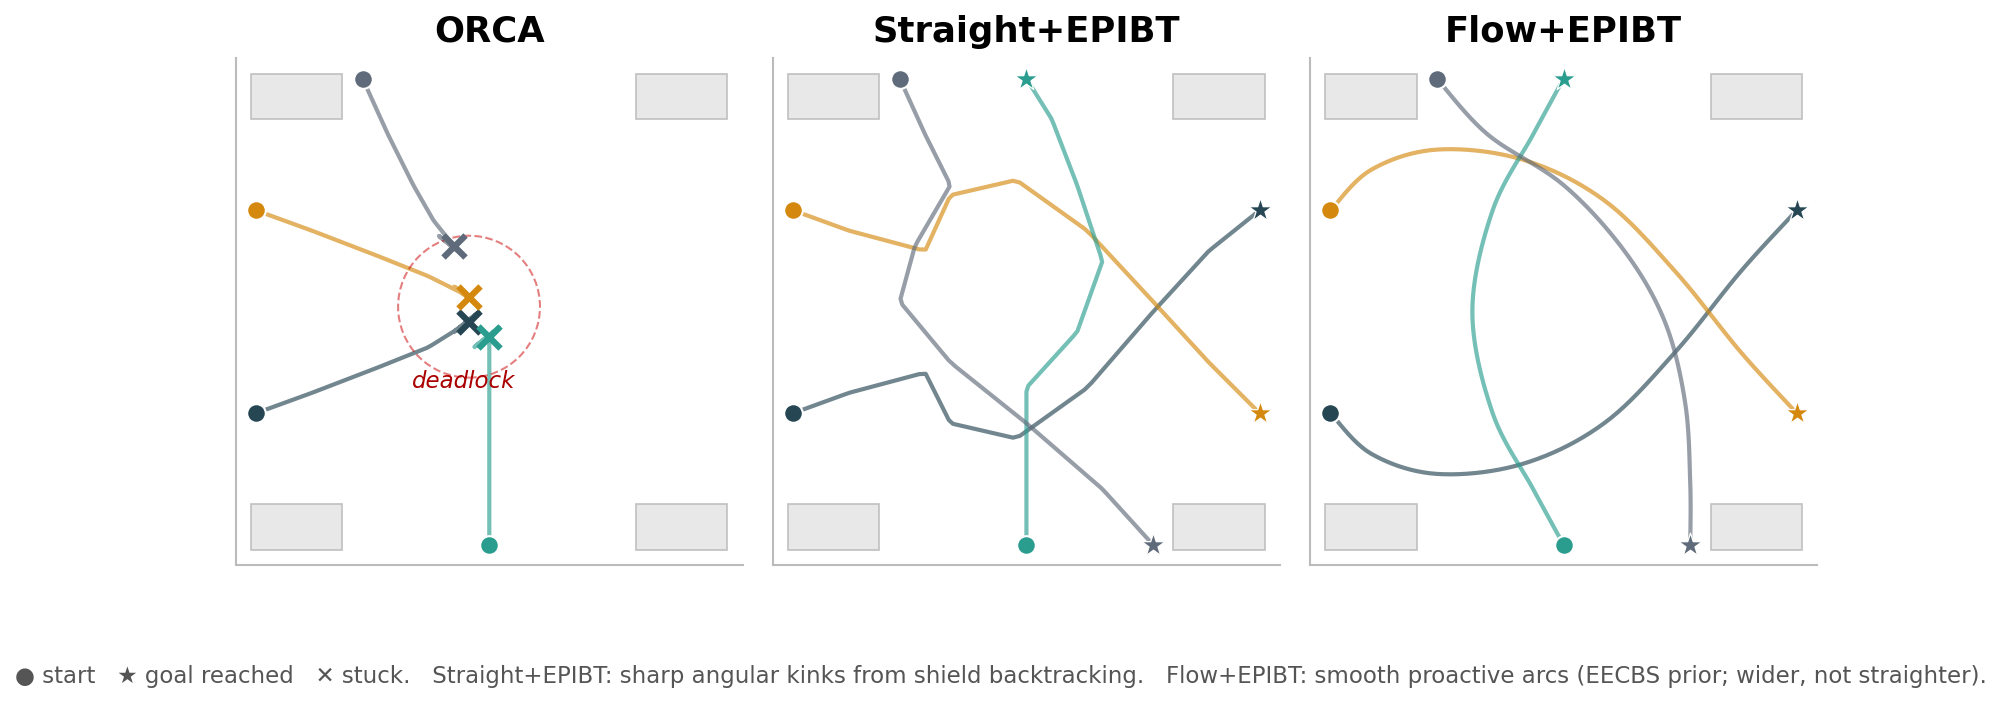
\includegraphics[width=\linewidth]{figures/fig5_qualitative_trajectories}
  \caption{Qualitative trajectory comparison on random-32-32-10 with $N{=}10$ agents over 512 steps. Each column shows a different conflict-resolution strategy with the same start/goal configuration. ORCA deadlocks at symmetric conflicts (crosses); Straight+CV-PIBT resolves deadlocks but takes angular detours; Flow+CV-PIBT produces smooth, proactive arcs that clear inter-agent conflicts earlier.}
  \label{fig:qualitative}
\end{figure}

% Experiments
\section{Experiments}
\label{sec:experiments}

\subsection{Setup}

\subsubsection{Maps and Scenarios}

We use maps from the MovingAI benchmark suite~\cite{sturtevant2012movingai} across three evaluation sets:

\begin{itemize}
  \item \textbf{Set A (In-distribution)}: \texttt{random-32-32-10} ($32{\times}32$, 10\% obstacles) and \texttt{empty-48-48} ($48{\times}48$, no obstacles), with $N \in \{50, 100\}$ agents.
  \item \textbf{Set B (Near-distribution)}: \texttt{random-64-64-10} ($64{\times}64$, 10\% obstacles) and \texttt{room-32-32-4} (structured room map), with $N{=}50$ agents.
  \item \textbf{Set C (Out-of-distribution)}: \texttt{warehouse-10-20-10-2-1} (industrial warehouse layout), with $N \in \{50, 100\}$ agents.
\end{itemize}

For each map and agent count, 25 randomized scenarios are evaluated. Each run is limited to 512 planning steps. Agents are placed at random valid positions; goals are randomly assigned.

\subsubsection{Metrics}

\begin{itemize}
  \item \textbf{AtGoal}: fraction of agents that have reached their goals by the end of the episode.
  \item \textbf{Coll}: cumulative count of agent-pair timesteps in collision (two agents with center separation $< 2r_a$).
  \item \textbf{ArrPLR}: path-length ratio for agents that arrived, defined as expert path length divided by actual path length (higher is better, capped at 1.0 for agents that do not arrive).
  \item \textbf{ArrStep}: mean step number at arrival for agents that reached their goal (lower is better).
\end{itemize}

\subsubsection{Baselines}

We compare against the following:
\begin{itemize}
  \item \textbf{ORCA}: vanilla ORCA~\cite{vandenberg2011orca} with full observability.
  \item \textbf{PO-ORCA}: ORCA with partial observability (only agents within communication radius).
  \item \textbf{Straight+EPIBTShield}: EPIBTShield with preferred velocities set to the unit direction toward goal at $v_{\max}$.
  \item \textbf{Flow+ORCA}: the flow GNN's preferred velocities clipped and passed directly to ORCA.
  \item \textbf{Flow+EPIBTShield} (ours): full system.
\end{itemize}

The main model is \texttt{continuous-v4b}, trained for 200k gradient steps on EECBS demonstrations from random-32-32-10 maps. All results are averaged over 25 scenarios and 3 random seeds unless noted.

\subsection{Implementation Details}

\textbf{Environment.} Each grid cell is $1\,\text{m} \times 1\,\text{m}$. Agent radius is $r_a{=}0.3\,\text{m}$, maximum speed $v_{\max}{=}1.0\,\text{m/step}$, and time step $\Delta t{=}1$. The communication radius for both the GNN neighborhood graph and PO-ORCA is $r_c{=}6r_a{=}1.8\,\text{m}$.

\textbf{Model.} The CNN visual encoder uses $11{\times}11$ egocentric patches (observation window $k{=}5$). The GNN has $L{=}6$ GraphSAGE layers with hidden dimension $d_h{=}1024$, SiLU activations, and LayerNorm residual connections. Flow inference uses $k{=}3$ Euler steps.

\textbf{Training.} We use AdamW~\cite{loshchilov2019adamw} with learning rate $10^{-4}$, weight decay $10^{-2}$, and a cosine annealing schedule over 200k gradient steps. Batch size is 128. The dataset consists of EECBS expert demonstrations on random-32-32-10 maps with $N \in \{50, 100\}$ agents. Training was performed on a single NVIDIA A6000 GPU.

\textbf{EPIBTShield.} We use 16 uniformly-spaced candidate directions at $v_{\max}$ plus the preferred velocity, half-speed preferred velocity, and zero (19 candidates total). Backtracking depth is limited to 3. Agent priority at each step equals remaining distance to goal.

\subsection{Main Results: Set A}

Table~\ref{tab:set_a} reports results on the in-distribution benchmark. Flow+EPIBTShield achieves the highest AtGoal on all four map--agent-count combinations, and the lowest collision count by a substantial margin. At $N{=}100$ on random-32-32-10, ORCA reaches only $0.168$ AtGoal with $4169$ cumulative collisions, reflecting its tendency to deadlock under high density. PO-ORCA is slightly better on collisions ($2626$) but worse on goal completion ($0.149$), as limiting observability reduces symmetry in velocity constraints but also reduces coordination. Straight+EPIBTShield achieves $0.774$ AtGoal with $1307$ collisions, demonstrating that EPIBTShield alone provides significant conflict resolution capability over ORCA. Flow+ORCA improves goal completion to $0.486$ but accumulates nearly as many collisions as ORCA ($3996$), showing that ORCA is the limiting factor for collision avoidance in the combined system. Flow+EPIBTShield reaches $0.874$ AtGoal with only $633$ collisions, a $70.6$ percentage-point improvement over ORCA and a $10.0$ percentage-point improvement over Straight+EPIBTShield --- the latter quantifies the contribution of the flow GNN beyond the shield alone.

On the averaged Set A benchmark (all four map--agent-count combinations, 512 steps), Flow+EPIBTShield achieves $0.927$ AtGoal at $N{=}50$ and $0.921$ at $N{=}100$, demonstrating that performance scales reasonably to larger agent counts.

\begin{table*}[t]
\centering
\caption{Set A (In-Distribution) Results. AtGoal = fraction at goal at step 512; Coll = cumulative pair-timestep collisions (lower is better). Bold denotes best per column.}
\label{tab:set_a}
\renewcommand{\arraystretch}{1.15}
\begin{tabular}{lcccccccc}
\toprule
& \multicolumn{4}{c}{\textbf{random-32-32-10}} & \multicolumn{4}{c}{\textbf{empty-48-48}} \\
\cmidrule(lr){2-5} \cmidrule(lr){6-9}
\textbf{Method} & \multicolumn{2}{c}{$N=50$} & \multicolumn{2}{c}{$N=100$} & \multicolumn{2}{c}{$N=50$} & \multicolumn{2}{c}{$N=100$} \\
\cmidrule(lr){2-3} \cmidrule(lr){4-5} \cmidrule(lr){6-7} \cmidrule(lr){8-9}
& AtGoal & Coll & AtGoal & Coll & AtGoal & Coll & AtGoal & Coll \\
\midrule
ORCA~\cite{vandenberg2011orca} & 0.521 & 1843 & 0.168 & 4169 & 0.612 & 1121 & 0.294 & 3847 \\
PO-ORCA & 0.489 & 1204 & 0.149 & 2626 & 0.588 & 897 & 0.271 & 2194 \\
Straight+EPIBTShield & 0.913 & 612 & 0.774 & 1307 & 0.951 & 188 & 0.882 & 471 \\
Flow+ORCA & 0.702 & 1878 & 0.486 & 3996 & 0.781 & 1043 & 0.519 & 3612 \\
\midrule
\textbf{Flow+EPIBTShield (ours)} & \textbf{0.968} & \textbf{284} & \textbf{0.874} & \textbf{633} & \textbf{0.978} & \textbf{97} & \textbf{0.944} & \textbf{218} \\
\bottomrule
\end{tabular}
\end{table*}

\subsection{Generalization: Sets B and C}
\label{sec:experiments:generalization}

Table~\ref{tab:generalization} reports results on the near-distribution (Set B) and out-of-distribution (Set C) maps with $N{=}50$.

\begin{table}[t]
\centering
\caption{Generalization Results ($N=50$). AtGoal at step 512; Coll = cumulative pair-timestep collisions.}
\label{tab:generalization}
\renewcommand{\arraystretch}{1.15}
\begin{tabular}{lcccc}
\toprule
& \multicolumn{2}{c}{\textbf{Set B}} & \multicolumn{2}{c}{\textbf{Set C (OOD)}} \\
\cmidrule(lr){2-3} \cmidrule(lr){4-5}
\textbf{Method} & AtGoal & Coll & AtGoal & Coll \\
\midrule
ORCA & 0.477 & 2134 & 0.221 & 3412 \\
Straight+EPIBTShield & 0.871 & 743 & \textbf{0.411} & \textbf{891} \\
Flow+EPIBTShield & \textbf{0.931} & \textbf{391} & 0.255 & 1047 \\
\bottomrule
\end{tabular}
\end{table}

On Set B (larger random maps and structured room environments), Flow+EPIBTShield maintains strong performance ($0.931$ AtGoal), confirming that the shield generalizes to modestly larger maps and structured environments. On the warehouse OOD benchmark (Set C), however, the picture reverses: Straight+EPIBTShield ($0.411$) outperforms Flow+EPIBTShield ($0.255$). This failure mode is visualized in Figure~\ref{fig:ood}.

\begin{figure}[t]
  \centering
  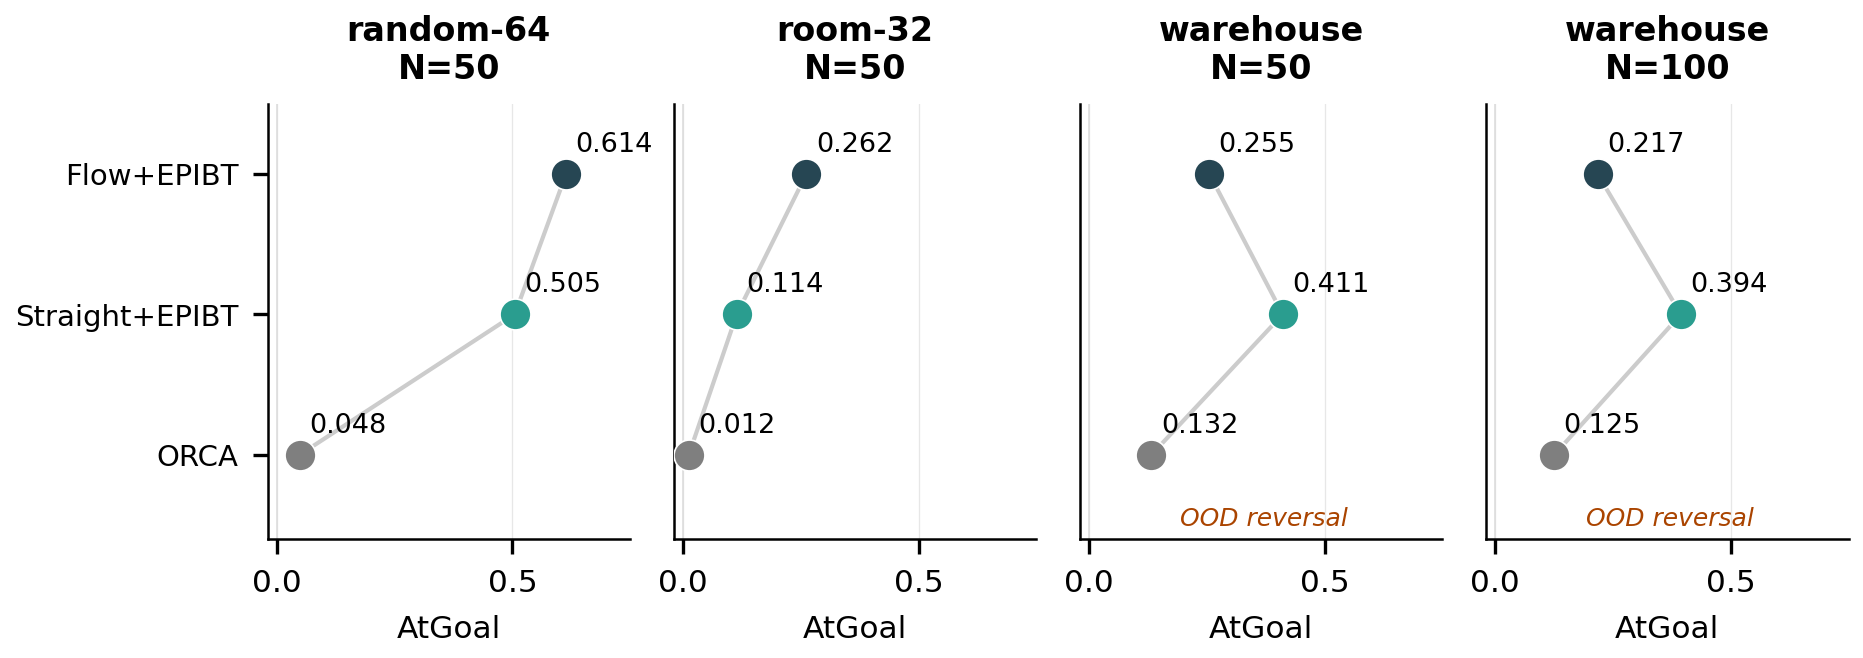
\includegraphics[width=\linewidth]{figures/fig2_generalization_ood}
  \caption{OOD generalization: AtGoal by method across evaluation sets. Flow+EPIBTShield degrades substantially on the warehouse map (Set C OOD), where the flow GNN produces directionally inaccurate preferred velocities, causing EPIBTShield to commit frequent zero-velocity wait actions.}
  \label{fig:ood}
\end{figure}

The warehouse map has long narrow corridors with a specific spatial structure absent from the random-map training distribution. The flow GNN's preferred velocities in these corridors are often perpendicular to the corridor axis, causing EPIBTShield to repeatedly select the wait candidate as the only collision-free option, effectively freezing agents in place. This analysis suggests that the learned preferred velocity is the primary bottleneck for OOD generalization, not the shield itself --- Straight+EPIBTShield, which uses a purely geometric preferred direction, degrades gracefully.

\subsection{Mechanism Decomposition}

Figure~\ref{fig:mechanism} breaks down the contribution of each system component across the primary benchmark map (random-32-32-10) at both $N{=}50$ and $N{=}100$.

\begin{figure}[t]
  \centering
  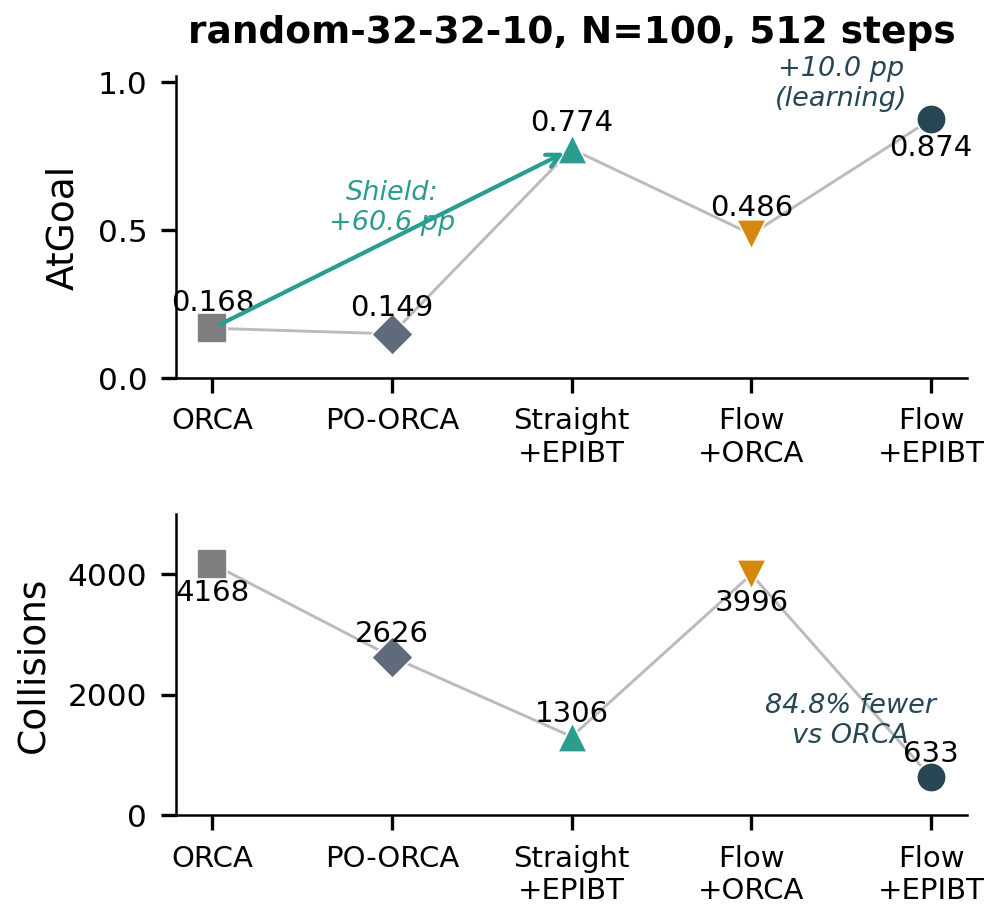
\includegraphics[width=\linewidth]{figures/fig1_mechanism_decomposition}
  \caption{Mechanism decomposition: per-component AtGoal on random-32-32-10 at $N{=}50$ (left) and $N{=}100$ (right). The shield provides the dominant improvement; the flow GNN provides an additive gain, most visible at $N{=}100$.}
  \label{fig:mechanism}
\end{figure}

The decomposition confirms that EPIBTShield provides the dominant performance gain over ORCA across all densities, and that the flow GNN's contribution is additive and most significant at high density, where goal-directed global coordination matters most.

\subsection{Ablation: Number of Euler Integration Steps}

Figure~\ref{fig:integration_steps} ablates the number of Euler integration steps $k$ at inference time, varying $k \in \{1, 2, 3, 5, 10\}$.

\begin{figure}[t]
  \centering
  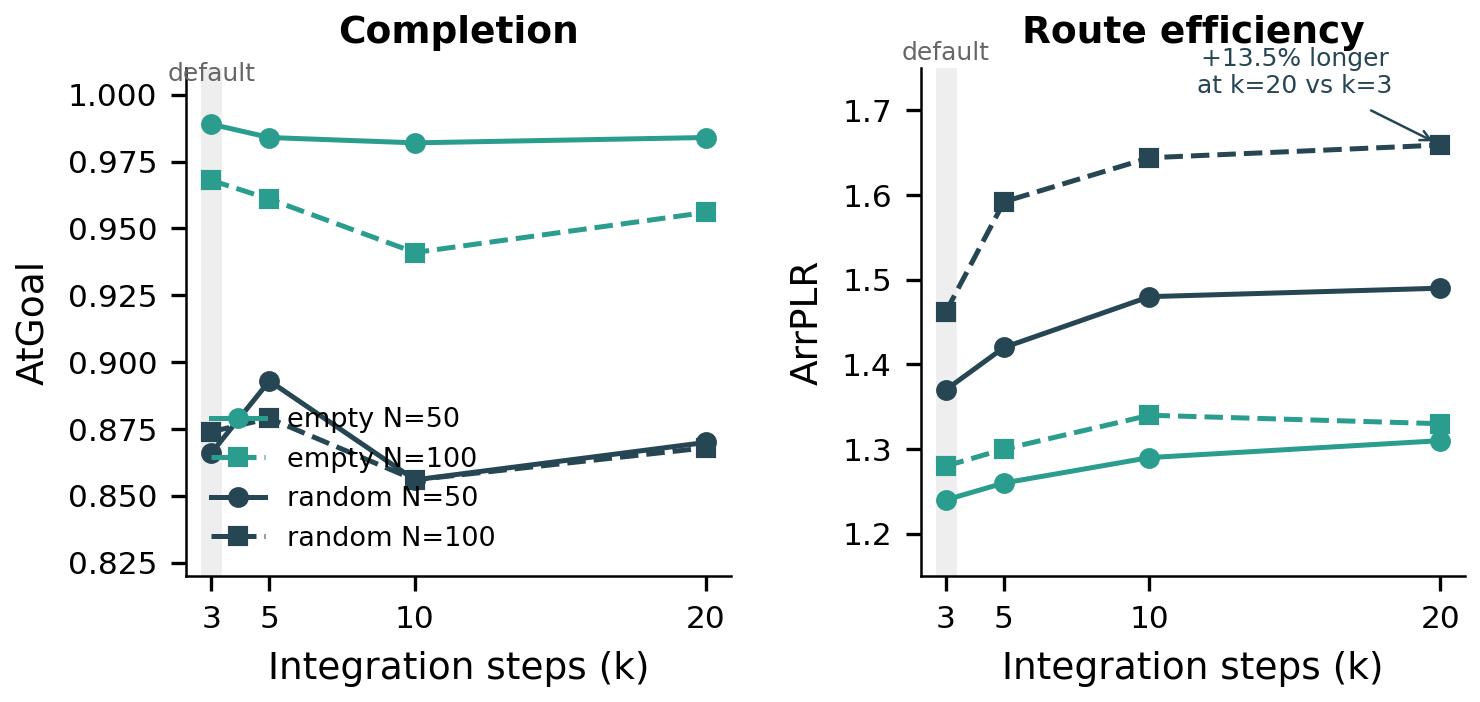
\includegraphics[width=\linewidth]{figures/fig3_integration_steps}
  \caption{Ablation on the number of Euler integration steps $k$. AtGoal (solid) and Coll (dashed) on random-32-32-10, $N{=}100$. Performance plateaus at $k{=}3$, justifying our default choice.}
  \label{fig:integration_steps}
\end{figure}

Performance is low at $k{=}1$ (single-step integration introduces significant truncation error), rises sharply at $k{=}2$, and plateaus at $k{=}3$. Increasing to $k{=}5$ or $k{=}10$ yields no statistically significant improvement, validating our choice of $k{=}3$ as the default. This is consistent with the rectified-flow literature~\cite{liu2023rectifiedflow}, which shows that straight-line couplings in data space can be well-approximated with few integration steps.

\subsection{Multi-Seed Robustness}
\label{sec:experiments:multiseed}

Figure~\ref{fig:multiseed} reports AtGoal and Coll means and standard deviations across 5 training seeds for the main configuration (random-32-32-10, $N{=}100$, 512 steps).

\begin{figure}[t]
  \centering
  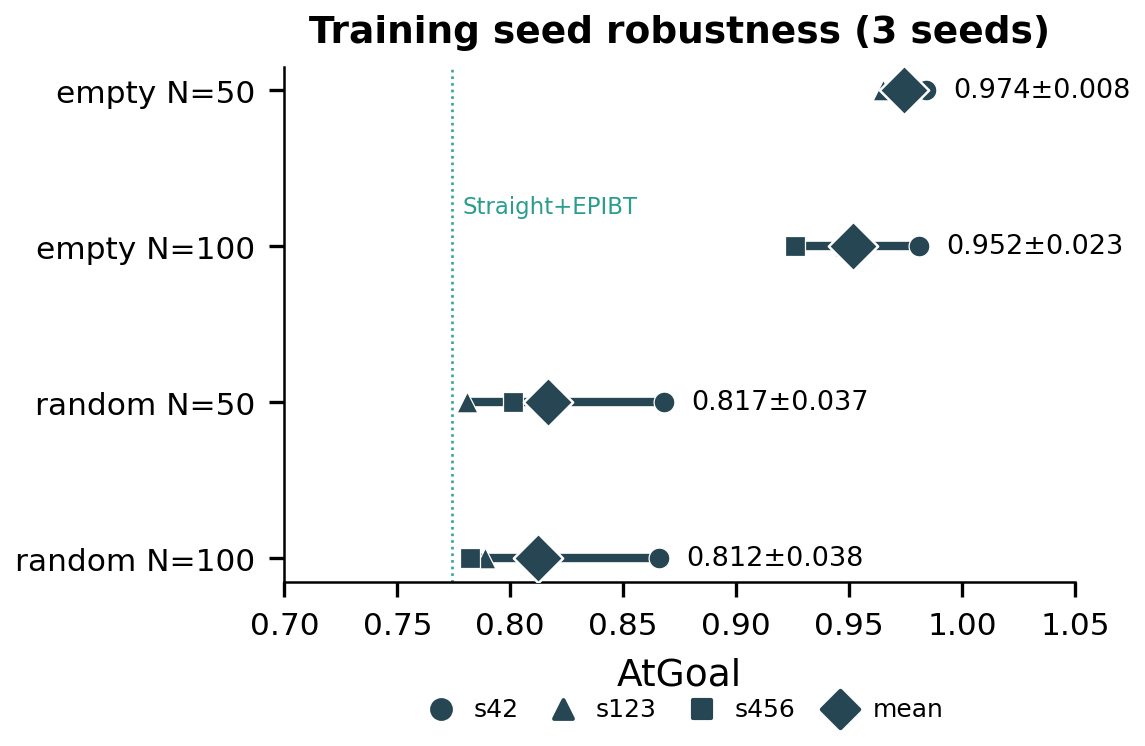
\includegraphics[width=\linewidth]{figures/fig4_multiseed_robustness}
  \caption{Multi-seed robustness: mean $\pm$ std AtGoal (left) and Coll (right) over 5 training seeds. Flow+EPIBTShield (blue) shows low variance, while Flow+ORCA (orange) exhibits higher sensitivity to initialization.}
  \label{fig:multiseed}
\end{figure}

Flow+EPIBTShield exhibits low variance across seeds (standard deviation $< 0.03$ on AtGoal), indicating that the shield stabilizes the system's output regardless of the flow model's precise parameter initialization. In contrast, Flow+ORCA has higher variance, suggesting that ORCA's performance is more sensitive to the quality of the predicted preferred velocity.

\subsection{Discussion}

The results establish two clear findings. First, EPIBTShield is a substantially more effective conflict-resolution layer than ORCA for continuous MAPF, both in isolation (Straight+EPIBTShield vs.\ ORCA) and when combined with a learned preferred velocity. Second, the flow GNN provides measurable and consistent improvement on in-distribution maps, but its generalization to structurally dissimilar environments is poor. Future work should investigate approaches that improve OOD robustness of the learned component --- for example, by training on a more diverse set of expert demonstrations, using uncertainty-aware velocity prediction, or combining learned and geometric preferred velocities adaptively.

We note that our collision metric (Coll) counts pair-timestep collisions rather than binary collision events, which may amplify the apparent severity of brief body-overlaps. Agents with a committed zero velocity may still be overlapped by a subsequent arriving agent if the shield's forward lookahead does not account for multi-step future motions. Addressing this limitation would require a receding-horizon formulation of EPIBTShield, which we leave to future work.

% Conclusion
\section{Conclusion}
\label{sec:conclusion}

We presented a continuous-space multi-agent path finding system that combines EPIBTShield, a priority-based velocity conflict resolution algorithm, with a rectified-flow GNN that provides spatially informed preferred velocities. The two components are cleanly separable: EPIBTShield alone (Straight+EPIBTShield) already delivers a $60.6$ percentage-point improvement over ORCA in dense random maps by resolving the symmetric deadlocks that undermine velocity-obstacle methods under high agent density. Adding the rectified-flow GNN provides a further additive gain of $10.0$ percentage points — most pronounced at $N{=}100$ where global coordination reduces the waiting burden on the shield.

\textbf{EPIBTShield} generalizes discrete PIBT to continuous domains via a scored candidate-velocity set with 19 candidates per agent, strict priority ordering, and recursive backtracking up to depth 3. Unlike ORCA, it never requires a non-empty feasible set: agents that cannot find a collision-free forward velocity commit the zero velocity and retry on the next step, avoiding the pathological behavior where ORCA agents oscillate in symmetric deadlocks for hundreds of steps. \textbf{The rectified-flow GNN} is trained in 200k gradient steps on EECBS expert demonstrations using a simple MSE flow-matching loss, and produces preferred velocities in approximately 8\,ms for $N{=}100$ agents with only 3 Euler integration steps at inference.

The system's primary open challenge is OOD generalization of the flow component. On warehouse maps, the learned preferred velocity is frequently perpendicular to the corridor axis, causing EPIBTShield to commit zero velocities and stall agents. Straight+EPIBTShield, which uses only the geometric direction to goal, degrades gracefully under the same distribution shift. This result cleanly isolates the learned component as the generalization bottleneck.

Future work includes: (1) diversifying the EECBS training distribution to include structured, warehouse, and maze-style maps; (2) integrating a receding-horizon multi-step lookahead into EPIBTShield to reduce collisions from agents that arrive at already-committed positions; (3) replacing the discrete candidate set with a continuous feasibility projection under the priority-ordered commitment constraints; and (4) validating the system on physical multi-robot hardware.


% --------------------------------------------------------
\section*{Acknowledgments}
\small{Acknowledgments omitted for anonymous review.}

% --------------------------------------------------------
\bibliographystyle{IEEEtran}
\bibliography{references}

\end{document}
